% This file is the main document file for the JPC 2015 TTECTrA paper
\documentclass[]{aiaa-tc} % insert '[draft]' option to show overfull boxes

\usepackage{mathtools,amssymb}

\usepackage{gensymb}

\usepackage{array,multirow,rotating}
\usepackage{ifthen}
\usepackage{graphicx}
\usepackage{varioref}% smart page, figure, table, and equation referencing     
\usepackage{wrapfig}% wrap figures/tables in text (i.e., Di Vinci style)
\usepackage{threeparttable}% tables with footnotes
\usepackage{dcolumn}% decimal-aligned tabular math columns
 \newcolumntype{d}{D{.}{.}{-1}}
\usepackage{nomencl}% nomenclature generation via makeindex
\usepackage{makeidx}
 \makenomenclature
\usepackage{subfigure}% subcaptions for subfigures
\usepackage{subfigmat}% matrices of similar subfigures, aka small mulitples
\usepackage{fancyvrb}% extended verbatim environments
 \fvset{fontsize=\footnotesize,xleftmargin=2em}
\usepackage{lettrine}% dropped capital letter at beginning of paragraph
%\usepackage[dvips]{dropping}% alternative dropped capital package
\usepackage{hyperref}% hyperlinks [must be loaded after dropping]

\hypersetup{
  colorlinks   = true, %Colours links instead of ugly boxes
  urlcolor     = black, %Colour for external hyperlinks
  linkcolor    = black, %Colour of internal links
  citecolor   = black %Colour of citations
}

\graphicspath{ {./images/} }

\title{Evaluating the Effect of Actuator Dynamics in Variable Area Fan Nozzle on
 Gas Turbine Control}

\author{
 Metin F. Ozcan\thanks{Graduate Research Assistant, Aerospace Systems 
 Design Laboratory (ASDL), 275 Ferst Drive NW, Atlanta, GA 30332-0150, and 
 AIAA Student Member.}
 \ , Christopher Perullo\thanks{Research Engineer I, ASDL, and AIAA Member.}
 \ , Jimmy C. Tai\thanks{Senior Research Engineer, ASDL, and AIAA Member.} 
 \ , and Dimitri N. Mavris\thanks{Boeing Regents Professor of Advanced 
 Aerospace Systems Analysis, Director at ASDL, and AIAA Fellow.}  \\
 {\normalsize\itshape School of Aerospace Engineering, Georgia Institute of 
 Technology, Atlanta, GA, 30332}
\\ \\ \textit{and} \\ \\
 Jeffrey T. Csank\thanks{Research Engineer, Intelligent Control and Autonomy 
 Branch, and AIAA Member.}
 \ and Jeffrey C. Chin\thanks{Research Engineer, Propulsion Systems Analysis 
 Branch, and non-AIAA Member.}
\\
 {\normalsize\itshape NASA Glenn Research Center, Cleveland, OH, 44135}
}

% Data used by 'handcarry' option
\AIAApapernumber{YEAR-NUMBER}
\AIAAconference{Conference Name, Date, and Location}
\AIAAcopyright{\AIAAcopyrightD{YEAR}}

% Define commands to assure consistent treatment throughout document
\newcommand{\eqnref}[1]{(\ref{#1})}
\newcommand{\class}[1]{\texttt{#1}}
\newcommand{\package}[1]{\texttt{#1}}
\newcommand{\file}[1]{\texttt{#1}}
\newcommand{\BibTeX}{\textsc{Bib}\TeX}

\newcommand{\superscript}[1]{\ensuremath{^{\textnormal{#1}}}}
\newcommand{\subscript}[1]{\ensuremath{_{\textnormal{#1}}}}

%\RequirePackage{ifthen}
%\renewcommand{\nomgroup}[1]{%
%\ifthenelse{\equal{#1}{G}}{\item[\textbf{Greek Symbols}]}{
%\ifthenelse{\equal{#1}{S}}{\item[\textbf{Subscripts}]}{}}}

\begin{document}

\nomenclature{$EPR$}{Engine pressure ratio}
\nomenclature{$BPR$}{Bypass ratio}
\nomenclature{$N_f$}{Fan rotational speed, RPM}
\nomenclature{$N_c$}{Core rotational speed, RPM}
\nomenclature{$W_f$}{Fuel flow rate, lbm/s}
\nomenclature{$HPC$}{High pressure compressor}
\nomenclature{$LPC$}{Low pressure compressor}
\nomenclature{$TTECTrA$}{Tool for Turbine Engine Closed-Loop Transient 
Analysis}
\nomenclature{$SSA$}{Small single aisle}
\nomenclature{$NPSS$}{Numerical Propulsion System Simulation}
\nomenclature{$VAFN$}{Variable Area Fan Nozzle}

\maketitle

\begin{abstract}

Fan variable area nozzles (FVAN) can provide several benefits, such as improving propulsive efficiency, reducing jet noise, increasing fan surge margin, and controlling fan flutter margin, by changing the FVAN area as a function of the current operating condition.  For example, the top of climb flight condition requires a smaller FVAN area whereas take-off requires a larger FVAN area. When analyzing the performance at these steady-state flight conditions, the aforementioned benefits are observed.  However, the gas turbine must operate one steady-state condition to another safely throughout the mission to realize these benefits. 

During a transition from one steady-state condition to another, FVAN must respond in concert with shaft dynamics for performance and safety. If FVAN doesn't respond in accordance with the shaft dynamics, either thrust lapse or stall can occur at different flight conditions. The response time of FVAN depends strongly on actuator dynamics. Lighter actuators with shape memory alloys (SMA) were proposed instead of heavy and complex conventional hydraulic actuators to reduce the fuel burn penalty due to actuator weight when FVAN is on-board. The SMA actuators are more flexible and lighter, but also respond slower than the hydraulic actuators. Therefore, a gas turbine controller must compensate for the slower SMA actuators while controlling either one variable (fuel flow rate with FVAN schedule) or two variables (fuel flow rate and FVAN). This study aims to evaluate how current SMA actuators perform. %If current SMA actuators fail, how slow SMA actuators are acceptable will be determined.  %Do we need this last sentence?

The SMA actuators will be represented by a first order lag with representative time constant values selected from previous work on SMA actuators.  Using a gas turbine model in the small single aisle thrust class, closed-loop controllers will be developed for the cases where FVAN runs with a schedule and when a closed-loop controller directly regulates the FVAN area. Gas turbine transient performance for the two FVAN cases will be analyzed based on thrust lapse and stall margin. A signal with a series of steps, chops, and ramps will be used to test the two developed controllers. If the gas turbine cannot reach 98\% of maximum thrust in less than five seconds (FAA requirement) or keep a safe stall margin throughout the transient operation, the time constant will be reduced to determine the SMA actuator response required to meet the performance and safety requirements.
%A first order lag will represent the SMA actuators and the representative time constant values are selected from the literature on the SMA actuators. Using a gas turbine model in small single aisle thrust class, controllers will be developed for the cases where FVAN runs with a schedule or a controller changes FVAN area directly. Gas turbine transient performance for the two FVAN cases will be analyzed based on thrust lapse and stall margin. A signal with a series of steps, chops, and ramps will be used to test the two developed controllers. If the gas turbine cannot reach 98\% of maximum thrust in less than five seconds (FAA requirement) or keep a safe stall margin throughout the transient operation, the time constant will be reduced to observe how fast the SMA actuator needs to be for performance and safety.

\end{abstract}

\printnomenclature % creates nomenclature section produced by MakeIndex

\section{Introduction}

\lettrine[nindent=0pt]{V}{ariable} geometry components promise improvements in gas turbine performance and safety. However, the improvements come with more complexity in addition to a necessary trade-off study due to the additional actuator system. Fan variable area nozzle (FVAN) is an example for the improvements, increase in complexity, and trade-off. FVAN can improve propulsive efficiency, reduce jet noise, increase fan surge margin, and control fan flutter margin. On the other hand, the FVAN actuator system can reduce the efficiency increase due to its extra weight and the additional control variable - variable nozzle area - complicates the control system unless the variable nozzle area is scheduled. Scheduling does not provide better performance or safety than controlling directly. 

The cost and benefit analysis for FVAN has considered only steady state analysis so far. What the FVAN area should be at different steady state points can be determined to realize the mentioned benefits. For example, top of climb requires a smaller FVAN area whereas take-off requires a larger FVAN area. However, the gas turbine must switch from one steady state condition to another safely throughout the mission. During a transition from one steady state condition to another, FVAN must respond in concert with shaft dynamics for performance and safety. If FVAN doesn't respond in accordance with shaft dynamics, either thrust lapse or stall can occur at different flight conditions. 

How fast FVAN responds, depends strongly on how fast the actuator is. Lighter actuators with shape memory alloys (SMA) \cite{Mabe:2008,Mabe:2008:Paris} were proposed instead of heavy and complex conventional hydraulic actuators to reduce the fuel burn penalty due to actuator weight when FVAN is on-board. The SMA actuators are more flexible, lighter and slower than hydraulic actuators \cite{Rey:2001,Barooah:2002,Song:2007}. In addition, FVAN is a challenging application for SMA because above a certain temperature SMA material properties transition. Consequently, SMA actuator placement is important for FVAN application.  

Before determining where to place the SMA actuator, a gas turbine controller must compensate for the slower SMA actuators while controlling either one variable (fuel flow rate with FVAN schedule) or two variables (fuel flow rate and FVAN). This study aims to evaluate how current SMA actuators perform with their dynamic characters in transient operation. If current SMA actuators do not meet the performance and safety requirements, the second aim is to determine how fast SMA dynamics must be to meet the requirements.

The paper is divided into three parts. First, the gas turbine engine model used in this study will be presented. Particular details about FVAN modeling will be given in addition to multi-design point cycle design values. After covering the gas turbine model, the controller development processes for scheduled and controlled dynamic FVAN will be discussed. Finally, the results for the transient operation with the dynamic FVAN will be shown and analyzed. 

\section{Gas turbine modeling}

% This file includes the content for the Gas Turbine Modeling section

A high BPR separate flow turbofan model in small single aisle (SSA) thrust class 
was developed using multi-design point cycle design \cite{Schutte:2012:2,
Schutte:2012:1} in NPSS. This section will include details about the gas turbine 
design. In addition, modeling the VAFN will be discussed. The developed NPSS 
gas turbine model can also be included in a Matlab Simulink model for dynamic 
modeling or controller development.

\section{Controller development}

% This file includes the content for Controller Development section

The control system features a subset of a standard aircraft engine controller\cite{Csank:2010}, mainly focusing on the parts of the controller which affect the dynamic performance and excluding steady-state limiters.  The control system features a power management system designed to regulate the controlled variable and deliver the desired thrust and a protection logic system to ensures safe operation while transitioning from one power level to another.  The protection logic system will contain two limiters; an acceleration controller designed to prevent high pressure compressor surge and exceeding the high pressure turbine inlet temperature, and a deceleration controller to prevent low pressure compressor surge and prevent exceeding the minimum fuel to air ratio.  These controllers will still be integrating using the standard MAX-MIN logic.  This architecture, and the functionality to design a controller, is already available in the NASA MATLAB/Simulink environment in the Tool for Turbine Engine Closed-Loop Transient Analysis \cite{Csank:2014} (TTECTrA). For this study TTECTrA will be used to develop controllers and execute the dynamic simulations.

\section{Results}

% This file contains the content for the Results section

In this section the transient performance test results for the scheduled and controlled FVAN will be presented. Attention will be given to thrust lapses and fan stall margin. If the FVAN actuator turns out to be slow, time constant value will be decremented in steps to determine how fast the actuator must be for acceptable performance.

An NPSS model developed for a conventional high BPR turbofan in the SSA thrust class was linked with TTECTrA in Matlab Simulink through an S-function. The results for the controller development are presented here to illustrate how the work proposed in this paper will be shown.

The set points for the conventional high BPR turbofan are given in \autoref{fig:set_points}. The set point variables are $EPR$, $N_f$, $N_c$, and $Wf$ whereas the set point function is for net thrust. The set point functions are not exactly linear but they can be approximated with linear relations if necessary.  

% Set points figure
\begin{figure}[!htb]
    \begin{center}
    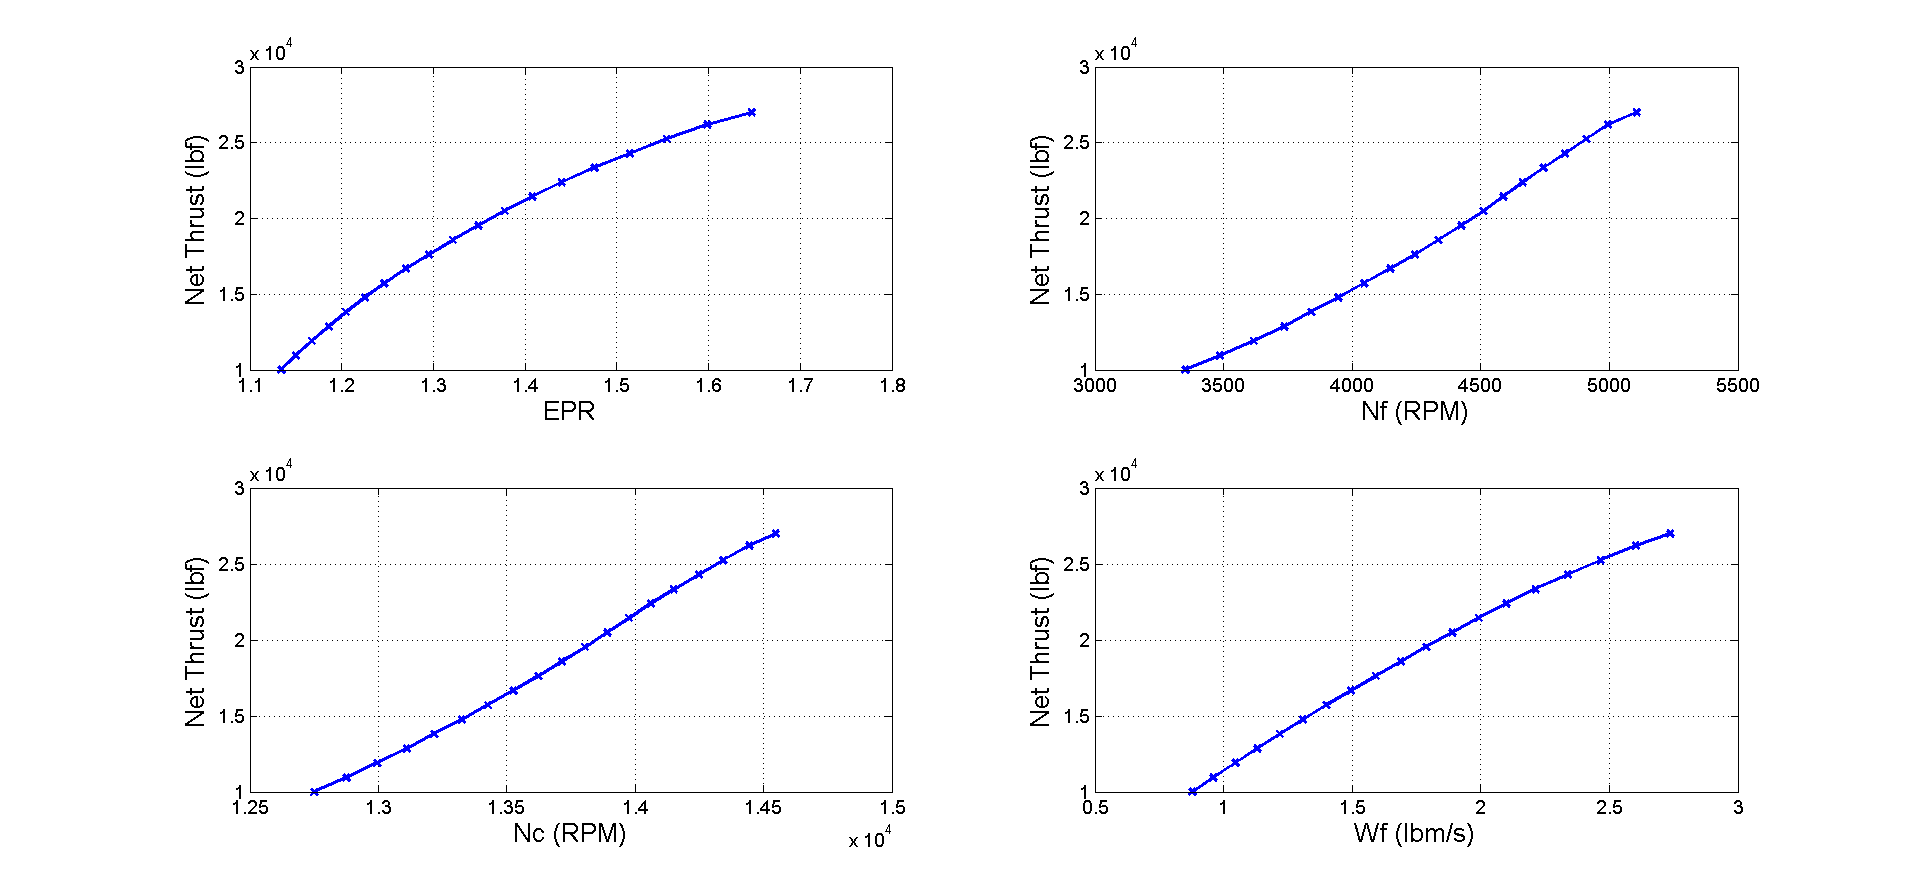
\includegraphics[width=\textwidth, height=\textheight,keepaspectratio]{set_points.png}
    \caption{Set points for the conventional high BPR turbofan}
    \label{fig:set_points}
    \end{center}
\end{figure}

\autoref{fig:acceleration_schedule} presents the acceleration schedule for the conventional high BPR turbofan. This schedule is used in the limiter for acceleration. The schedule was determined by running more and more demanding signals until the HPC stall margin limit was reached. 

% Acceleration schedule figure
\begin{figure}[!htb]
    \begin{center}
    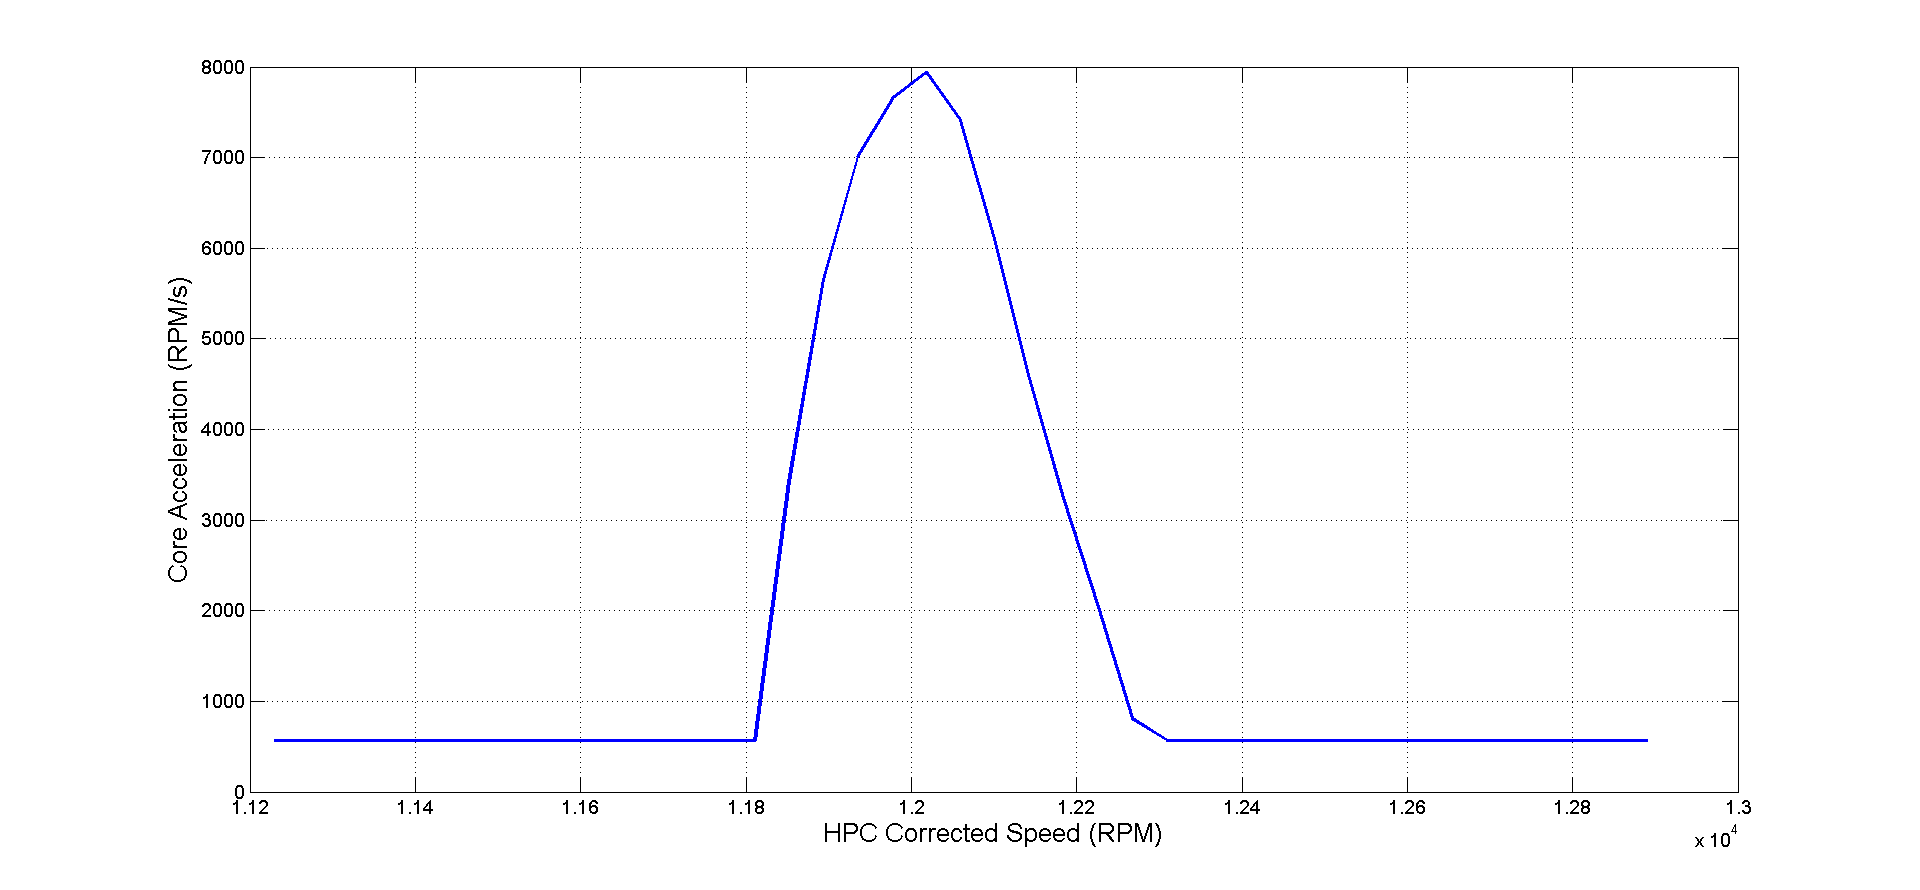
\includegraphics[width=\textwidth, height=\textheight,keepaspectratio]{acceleration_schedule.png}
    \caption{Acceleration schedule for the conventional high BPR turbofan}
    \label{fig:acceleration_schedule}
    \end{center}
\end{figure}

The conventional high BPR turbofan net thrust response for a signal with a series of steps, chops, and ramps is in \autoref{fig:net_thrust_response}. The controller follows the demand in an acceptable manner.

% Net thrust response figure
\begin{figure}[!htb]
    \begin{center}
    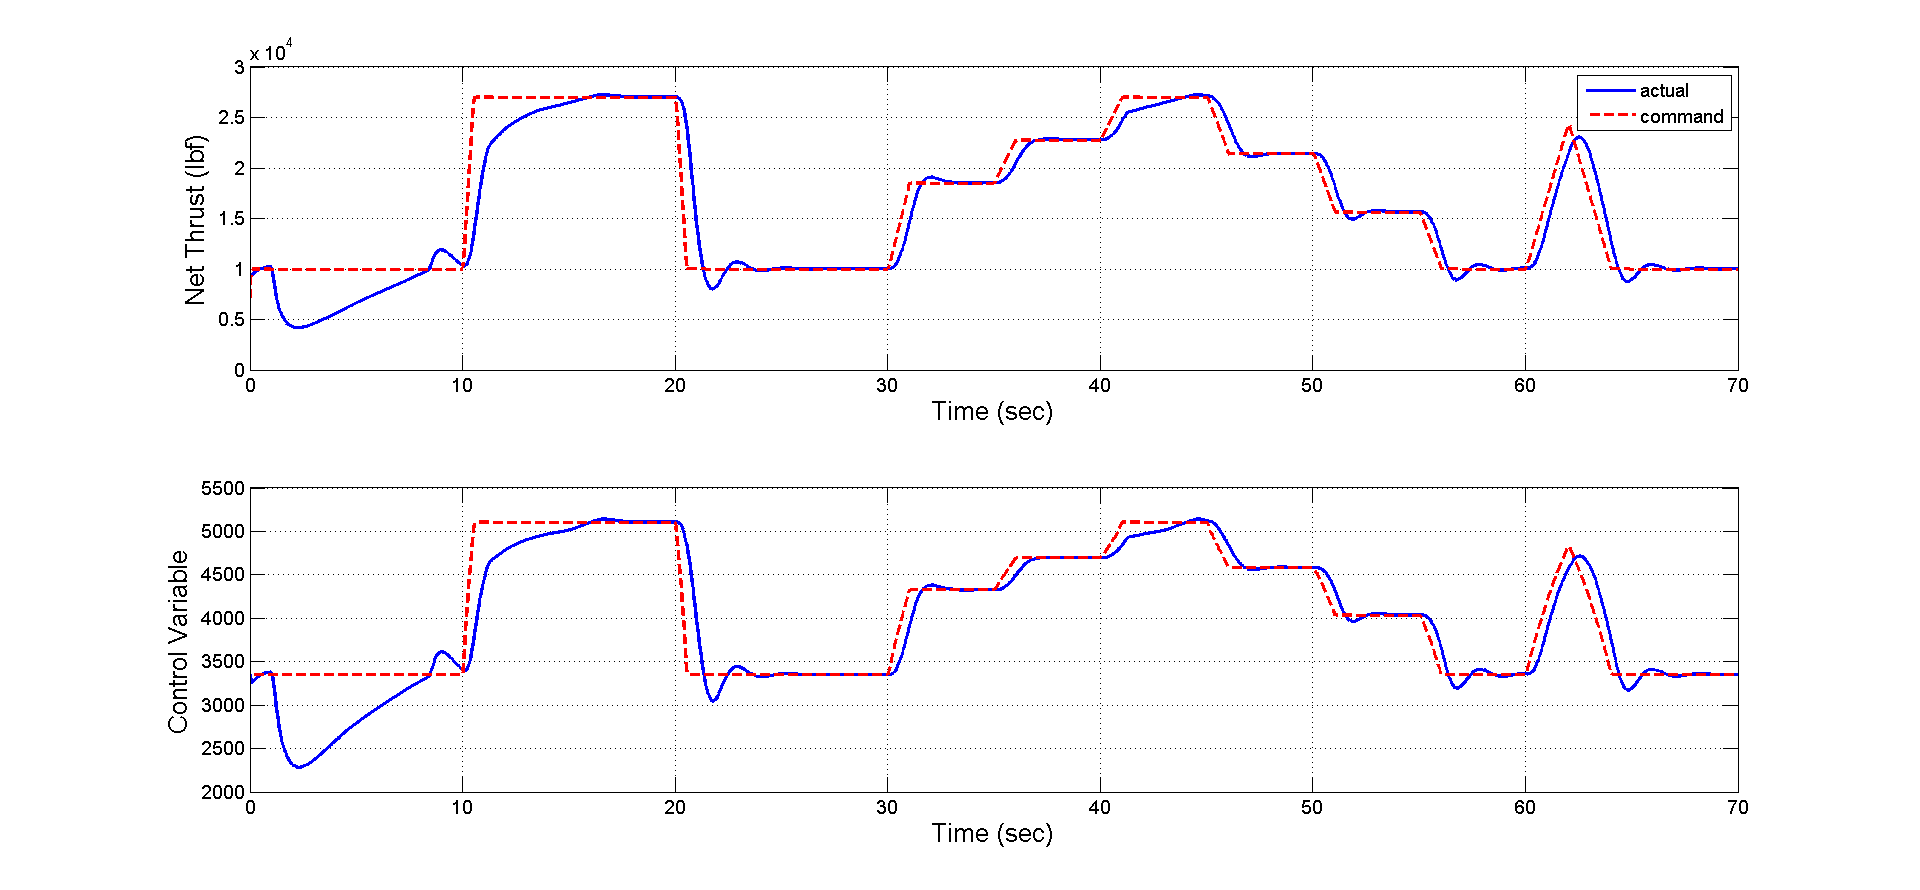
\includegraphics[width=\textwidth, height=\textheight,keepaspectratio]{net_thrust_response.png}
    \caption{Conventional high BPR turbofan net thrust response}
    \label{fig:net_thrust_response}
    \end{center}
\end{figure}

How the HPC surge margin changes throughout the net thrust response is shown in \autoref{fig:HPC_surge_margin}. The HPC stall margin did not come close to the limit throughout the entire transient. Also, \autoref{fig:HPC_surge_margin} gives the core acceleration against the acceleration schedule during the transient. The largest core acceleration recorded throughout the transient is less than a quarter of the maximum in the acceleration schedule. 

% HPC surge margin figure
\begin{figure}[!htb]
    \begin{center}
    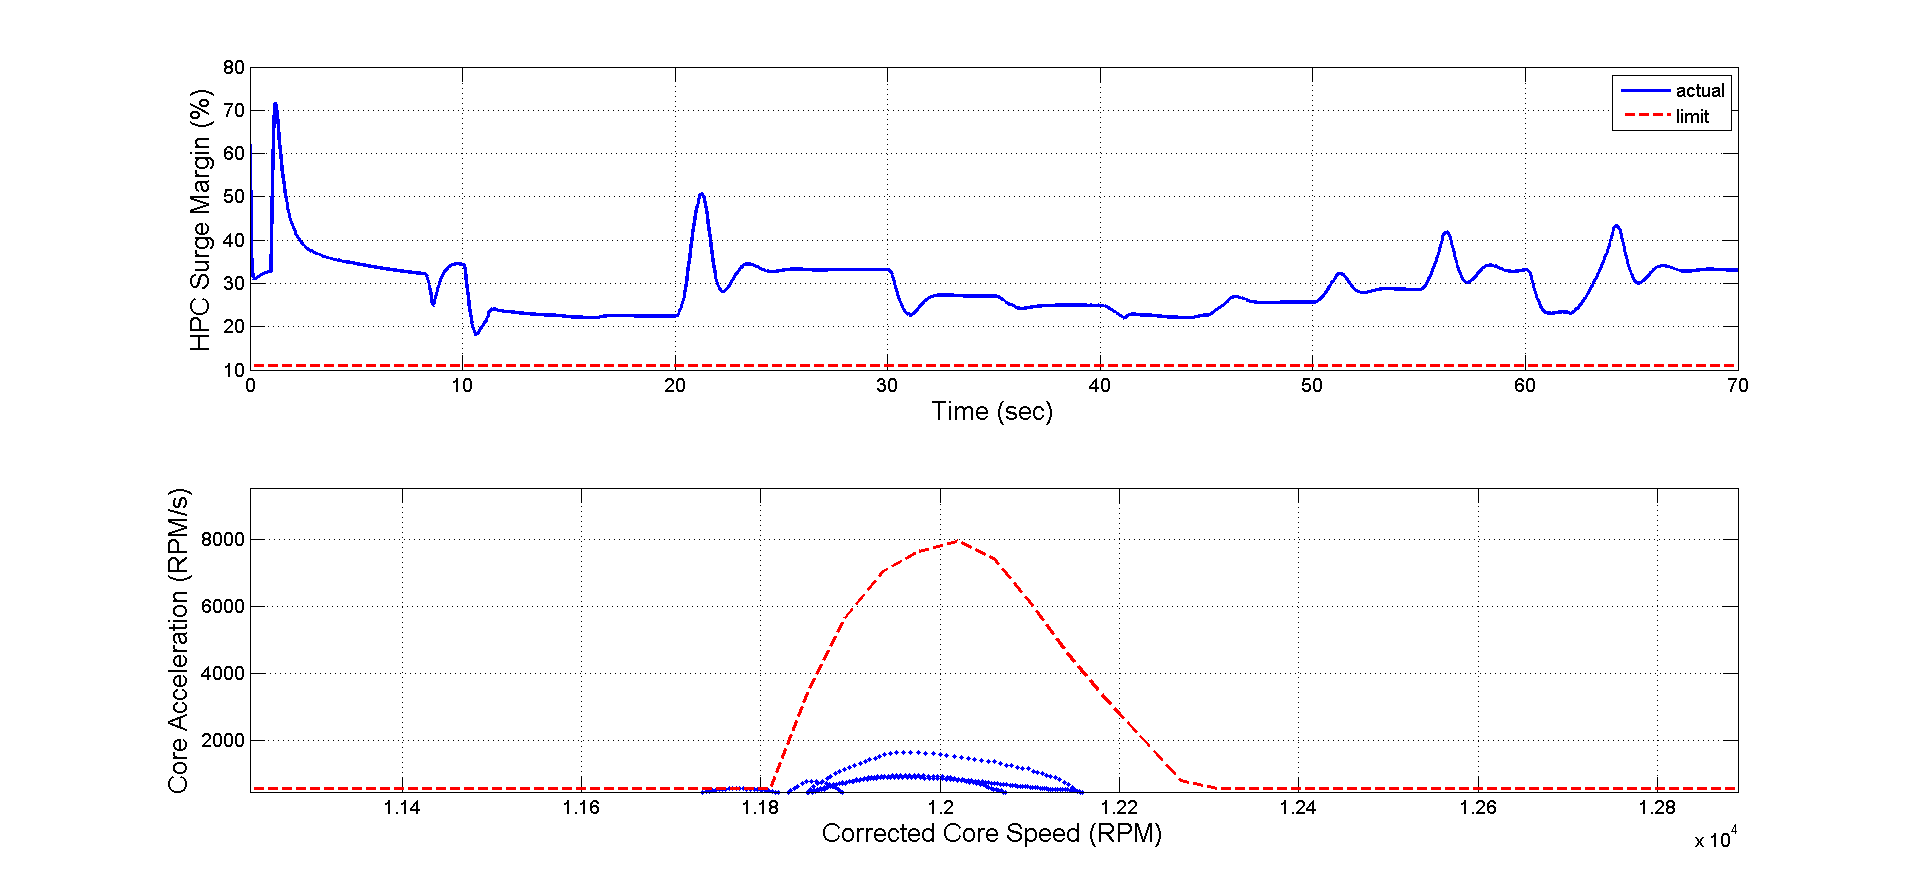
\includegraphics[width=\textwidth, height=\textheight,keepaspectratio]{HPC_surge_margin.png}
    \caption{Conventional high BPR turbofan HPC surge margin response}
    \label{fig:HPC_surge_margin}
    \end{center}
\end{figure}

Similar to the HPC case, \autoref{fig:LPC_surge_margin} shows how the LPC surge margin changed throughout the transient. The controller maintained the LPC stall margin more than 10\% during transient. \autoref{fig:LPC_surge_margin} also shows the change in combustor loading, $W_f/P_{s3}$, to measure combustor stability throughout the entire transient. The controller managed to keep the combustor loading above the limit in addition to the HPC and LPC stall margins.

% LPC surge margin figure
\begin{figure}[!htb]
    \begin{center}
    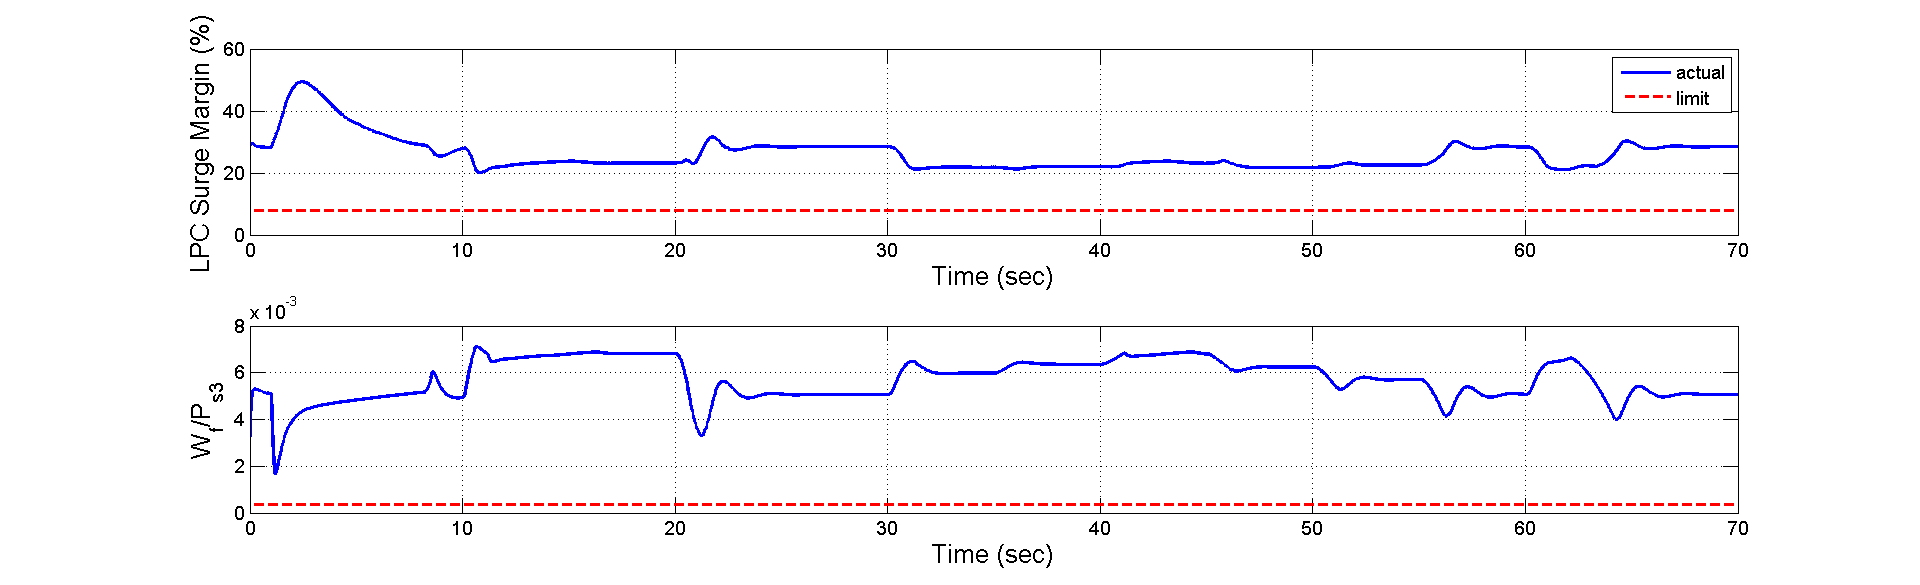
\includegraphics[width=\textwidth, height=\textheight,keepaspectratio]{LPC_surge_margin.png}
    \caption{Conventional high BPR turbofan LPC surge margin response}
    \label{fig:LPC_surge_margin}
    \end{center}
\end{figure}

\section{Conclusion}

Conclusion goes here.

% produces the bibliography section when processed by BibTeX
\bibliography{reference_database}
\bibliographystyle{aiaa}

\end{document} 